\documentclass[11pt,a4paper]{article}

\usepackage{titling}
\usepackage[hidelinks]{hyperref}
\usepackage{graphicx}
\usepackage{grffile}
\usepackage{float}
\usepackage{geometry}
\usepackage{listings}

\newcommand{\subtitle}[1]{
  \posttitle{
    \par\end{center}
    \begin{center}\large#1\end{center}
    \vskip0.5em}
}

\begin{document}
\title{Web Application User Manual}
\subtitle{ Git: \url{https://github.com/CodingInfinity/Benchmark-Service-Documentation} \\ GitHub Organisation: \url{https://github.com/CodingInfinity}}
\begin{figure}
			\centering
			
\includegraphics[height=230px]{../Images/CodingInfinity.png}
\end{figure}
\author{
	\textbf{The Client:} \\
	Ms Vreda Pieterse  \\
	Department of Computer Science \\
	University Of Pretoria
	\\
	\\
	\textbf{The Team:} \\
	Andrew Broekman		\emph{11089777}	\\
	Brenton Watt		\emph{14032644}	\\
	Fabio Loreggian		\emph{14040426}	\\
	Reinhardt Cromhout	\emph{14009936}	\\
}
\date{\textbf{May 2016}}

\maketitle
\thispagestyle{empty}
\pagebreak

\tableofcontents
\pagebreak
\section{Introduction}
This is the user manual for the Web Application. It gives a detailed guide surrounding individual how to
navigate and use each part of the system.

\section{Registration}
Upon starting up of the application and navigating to the home page, the user will be met with the screen seen in 
Figure \ref{fig:landPage}.
\begin{figure}[H]
	\begin{center}
		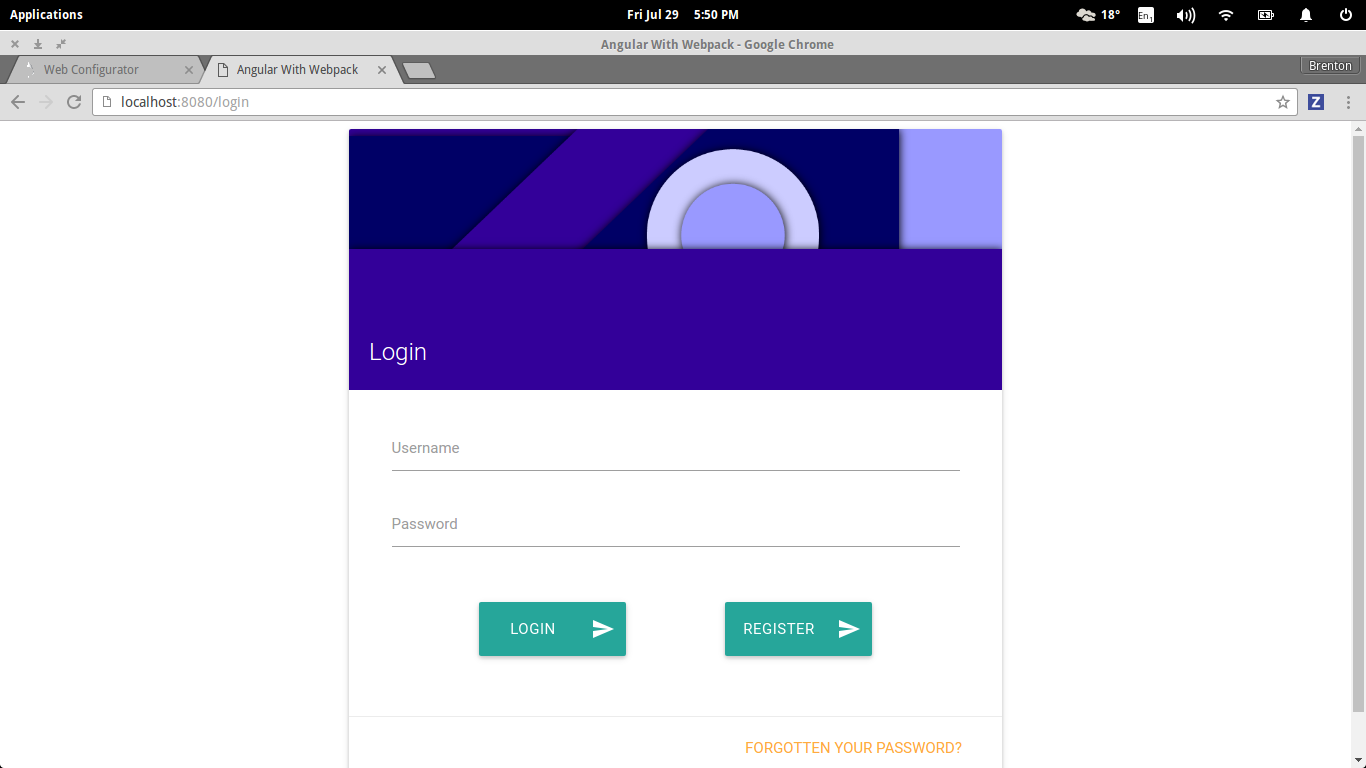
\includegraphics[scale=0.3]{../Images/User Manual/Landing Page.png}
		\caption{Landing Page}
		\label{fig:landPage}
	\end{center}  
\end{figure}

If the user has never made use of the system before, they should register themselves. Clicking on the "Register"
button will direct the user to the page seen in Figure \ref{fig:regPage}.
\begin{figure}[H]
	\begin{center}
		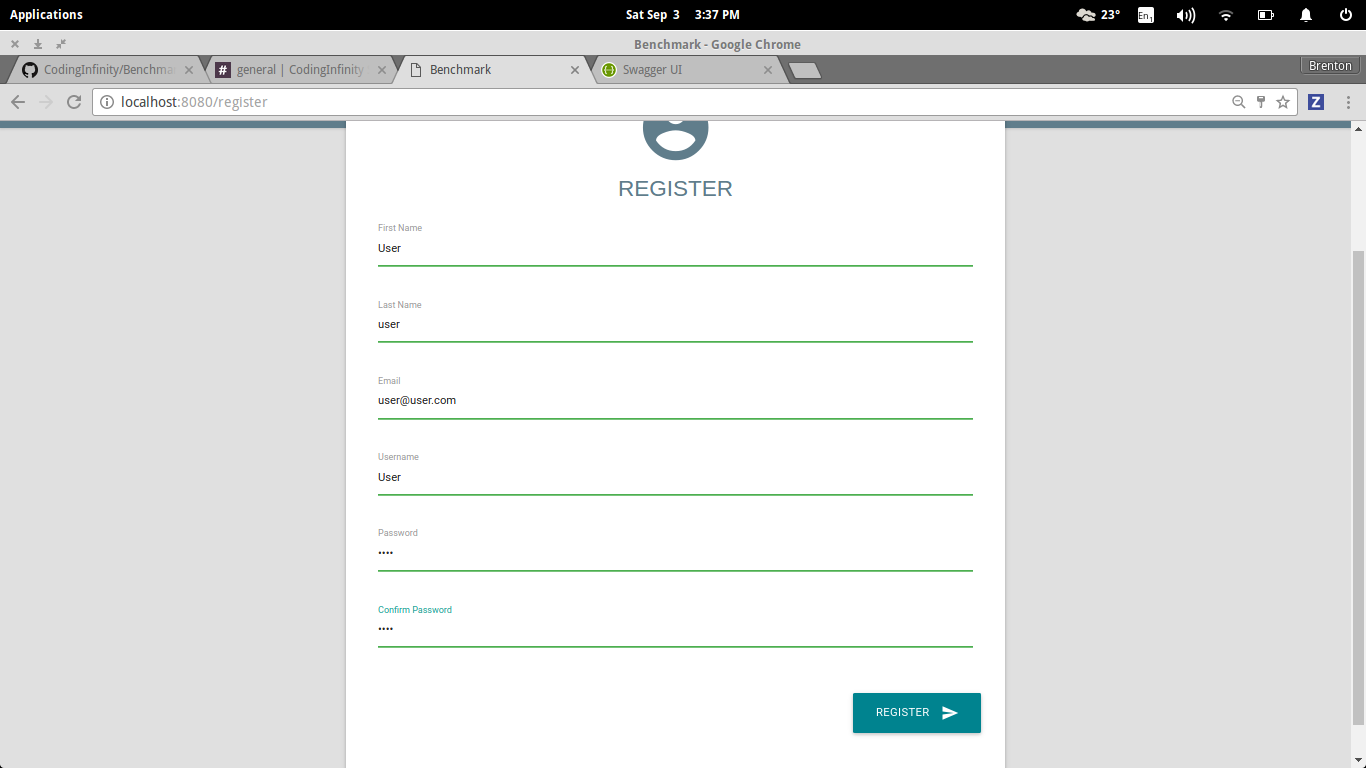
\includegraphics[scale=0.3]{../Images/User Manual/Registration Page.png}
		\caption{Registration Page}
		\label{fig:regPage}
	\end{center}  
\end{figure}

The user will then need to fill in their details accordingly. Once they have done this, they should click the "Submit" 
button. The user will then receive an email address at the address provided with a link that will allow them to activate
their account. When they click on the link they will arrive at a page as seen in Figure \ref{fig:activatePage}.
\begin{figure}[H]
	\begin{center}
		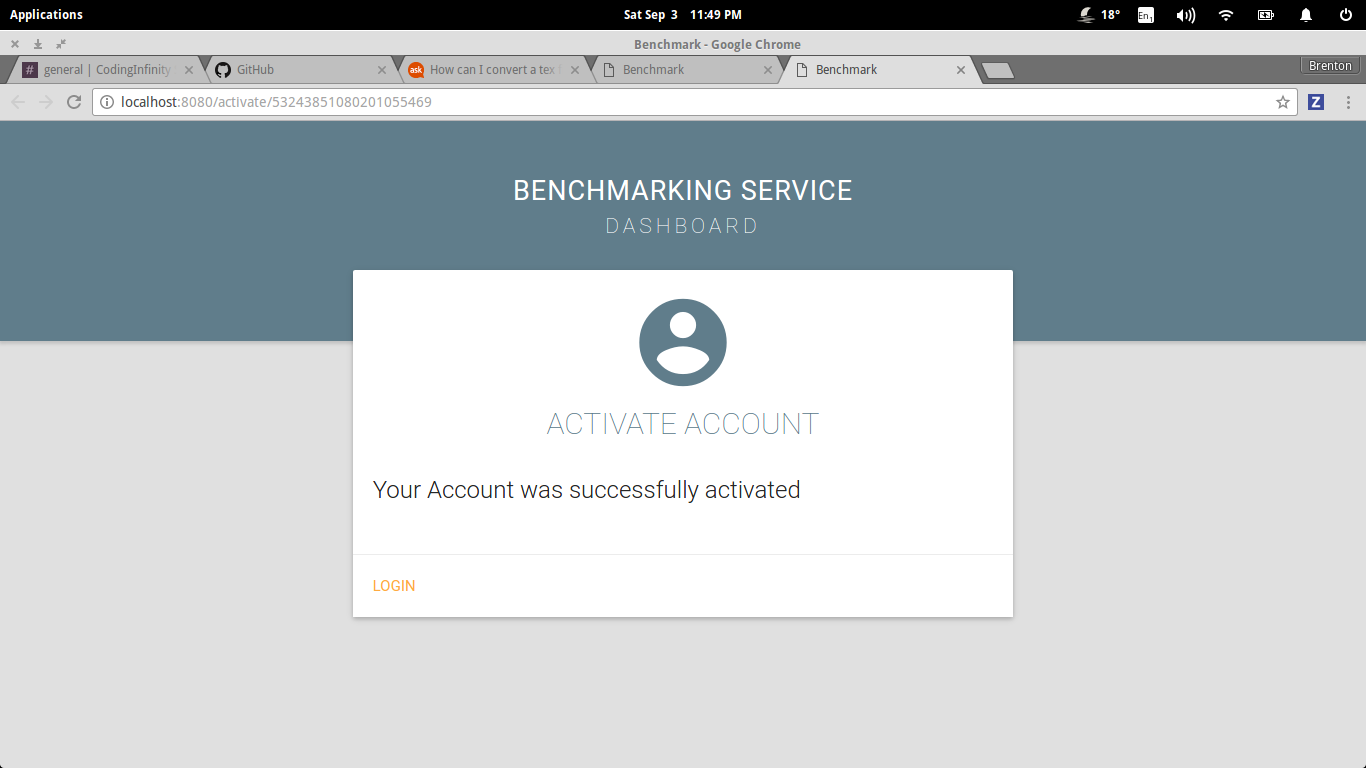
\includegraphics[scale=0.3]{../Images/User Manual/Activation Page.png}
		\caption{Activation Page}
		\label{fig:activatePage}
	\end{center}  
\end{figure}

\section{Sign In}
Once the user has registered and activated an account as detailed in the previous section or upon returning to the application,
they will be able to sign in by filling in their details as seen in Figure \ref{fig:signPage}.
\begin{figure}[H]
	\begin{center}
		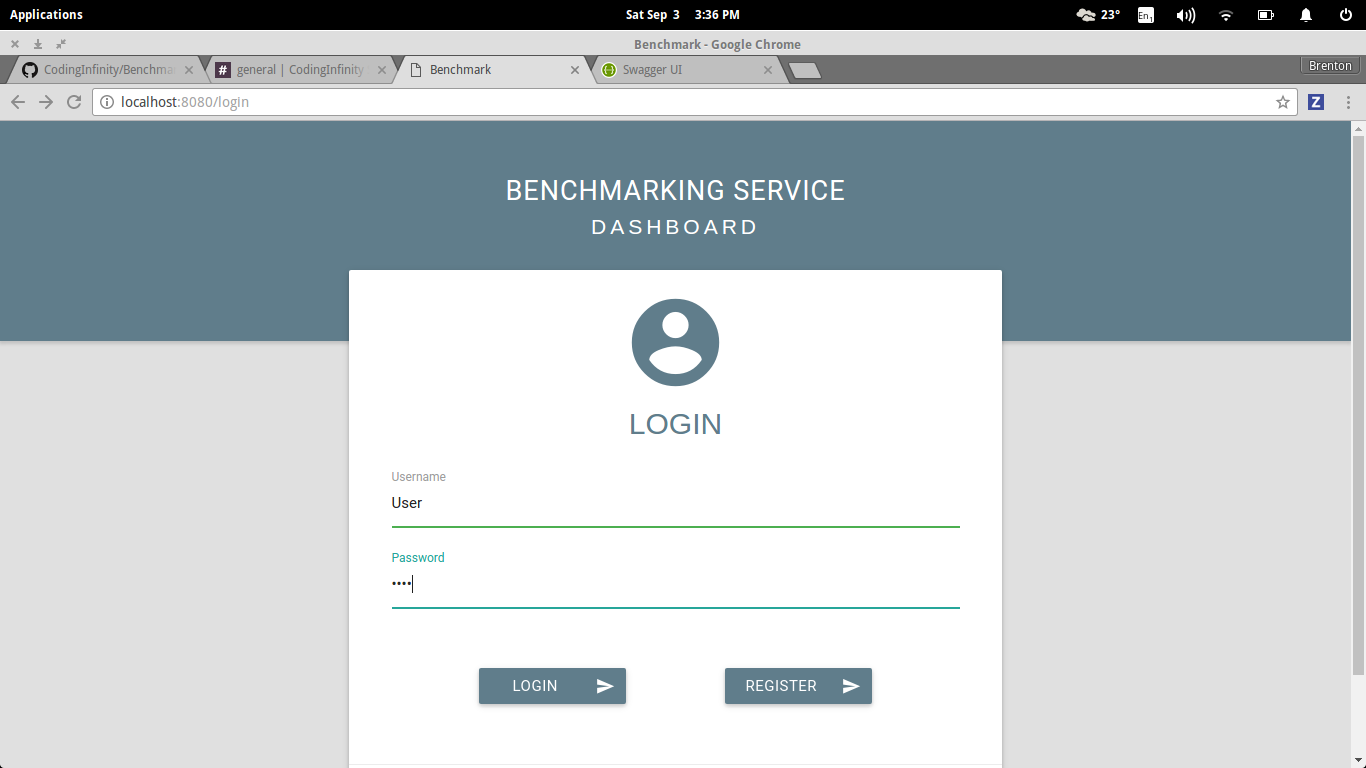
\includegraphics[scale=0.3]{../Images/User Manual/Sign in Page.png}
		\caption{Signing in}
		\label{fig:signPage}
	\end{center}  
\end{figure}

\section{Home}
Upon signing in, the user will arrive at the home page as seen in Figure \ref{fig:homePage}. From this page the user will be able 
to navigate throughout the application.
\begin{figure}[H]
	\begin{center}
		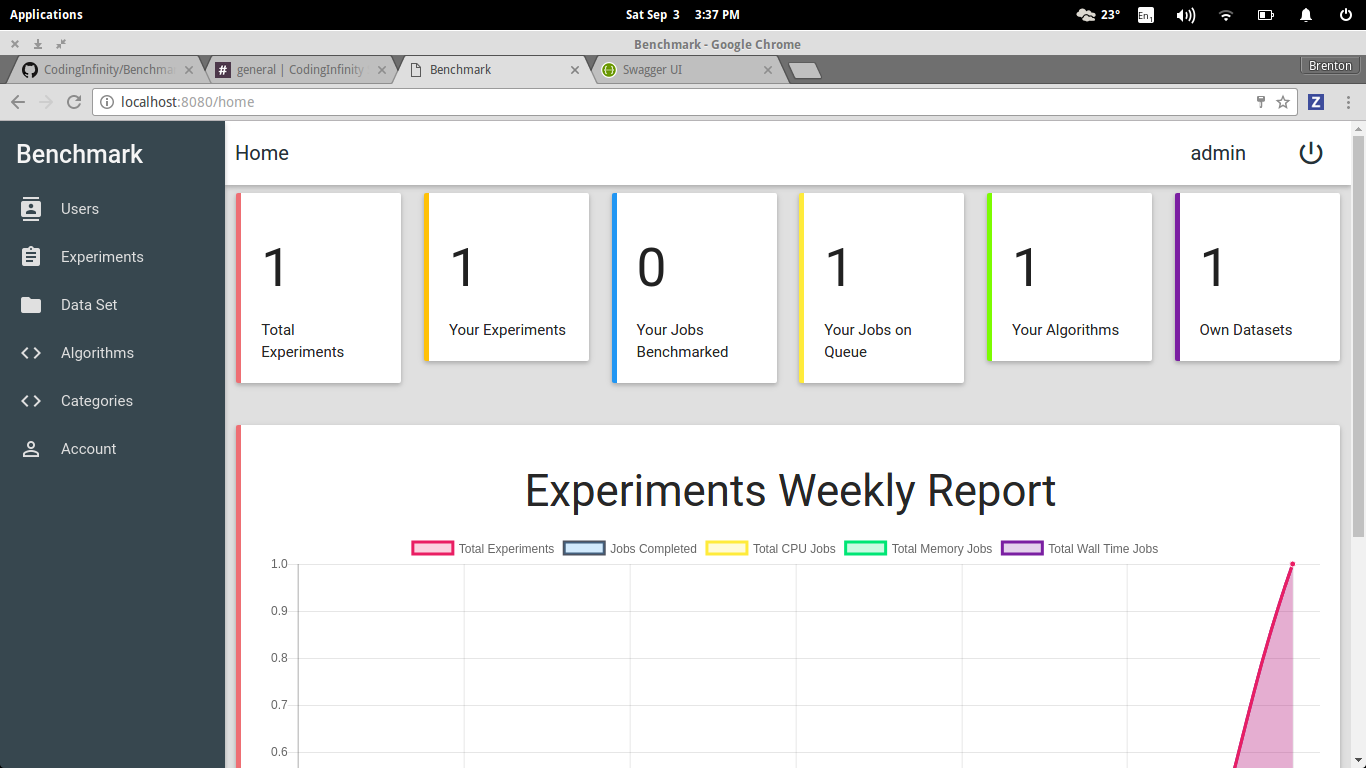
\includegraphics[scale=0.3]{../Images/User Manual/Home Page.png}
		\caption{Home Page}
		\label{fig:homePage}
	\end{center}  
\end{figure}
\section{Edit Profile}
In order to edit ones profile, click on the Account tab in the navigation bar and a drop down list will appear as seen in Figure \ref{fig:AccountPage}.
From there, click on the "Profile" option, which will take you to the Profile page as seen in Figure \ref{fig:ProfilePage}.
From here, the user can edit any of the options availible by clicking on the desired option and filling in the details as seen in
Figures \ref{fig:ProfilePage1}, \ref{fig:ProfilePage2}, \ref{fig:ProfilePage3}. Upon filling in the details, click the "Edit" button.
\begin{figure}[H]
	\begin{center}
		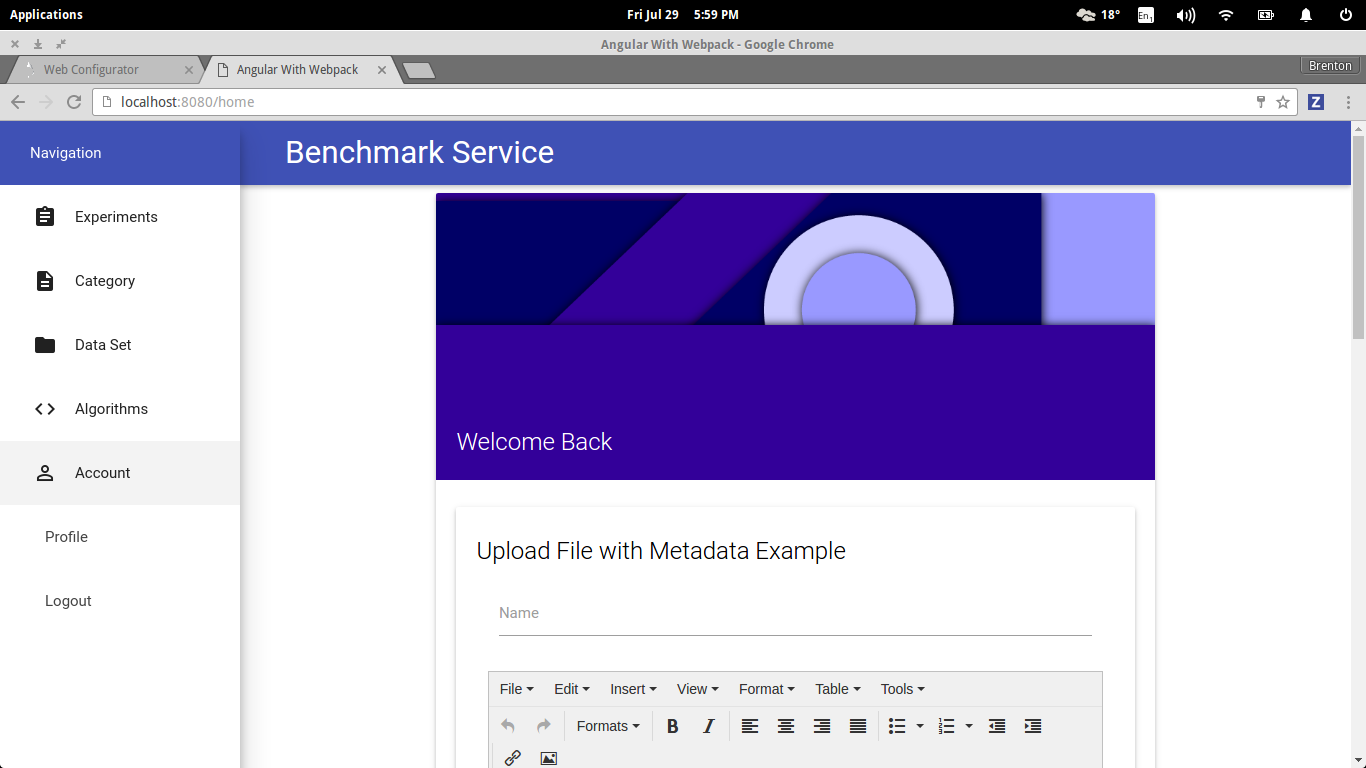
\includegraphics[scale=0.3]{../Images/User Manual/Account Page.png}
		\caption{Home Page with Account Drop down menu.}
		\label{fig:AccountPage}
	\end{center}  
\end{figure}
\begin{figure}[H]
	\begin{center}
		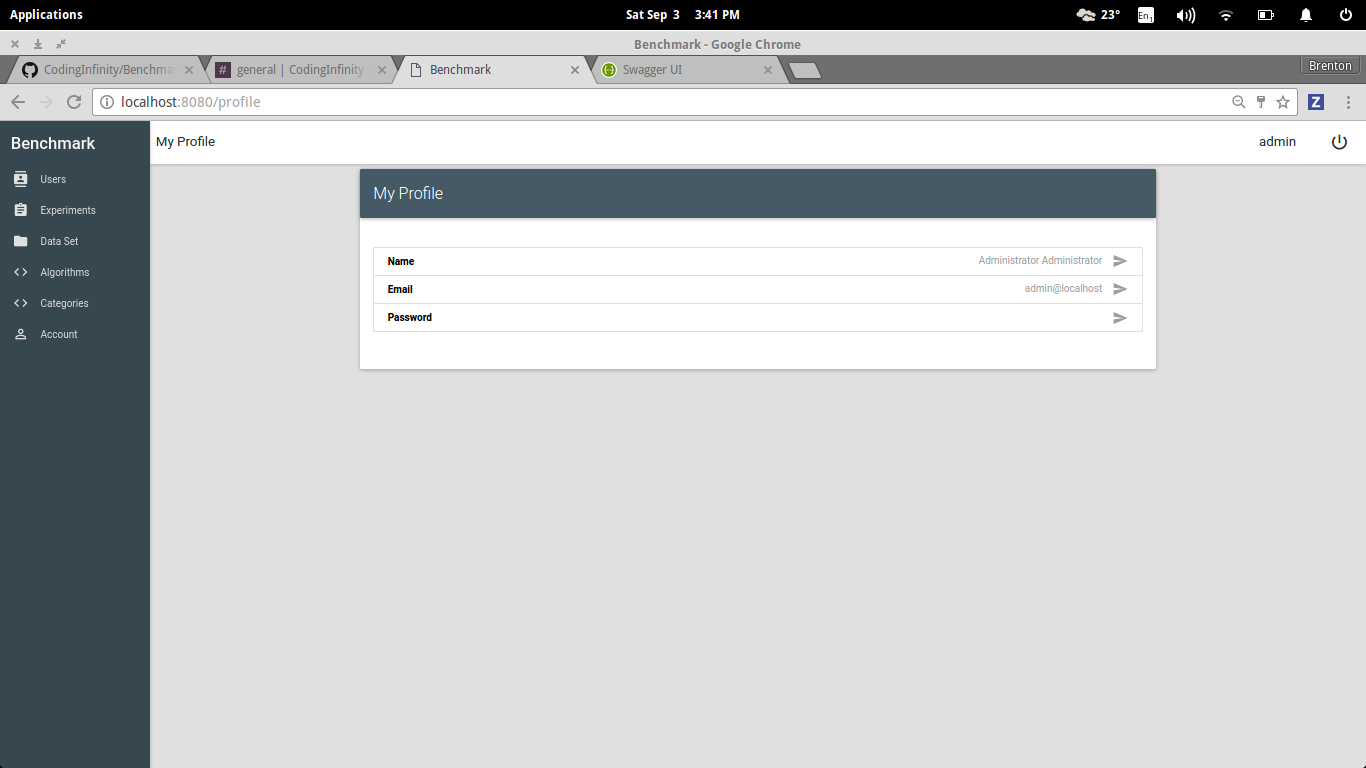
\includegraphics[scale=0.3]{../Images/User Manual/Profile Page.png}
		\caption{Profile Page}
		\label{fig:ProfilePage}
	\end{center}  
\end{figure}
\begin{figure}[H]
	\begin{center}
		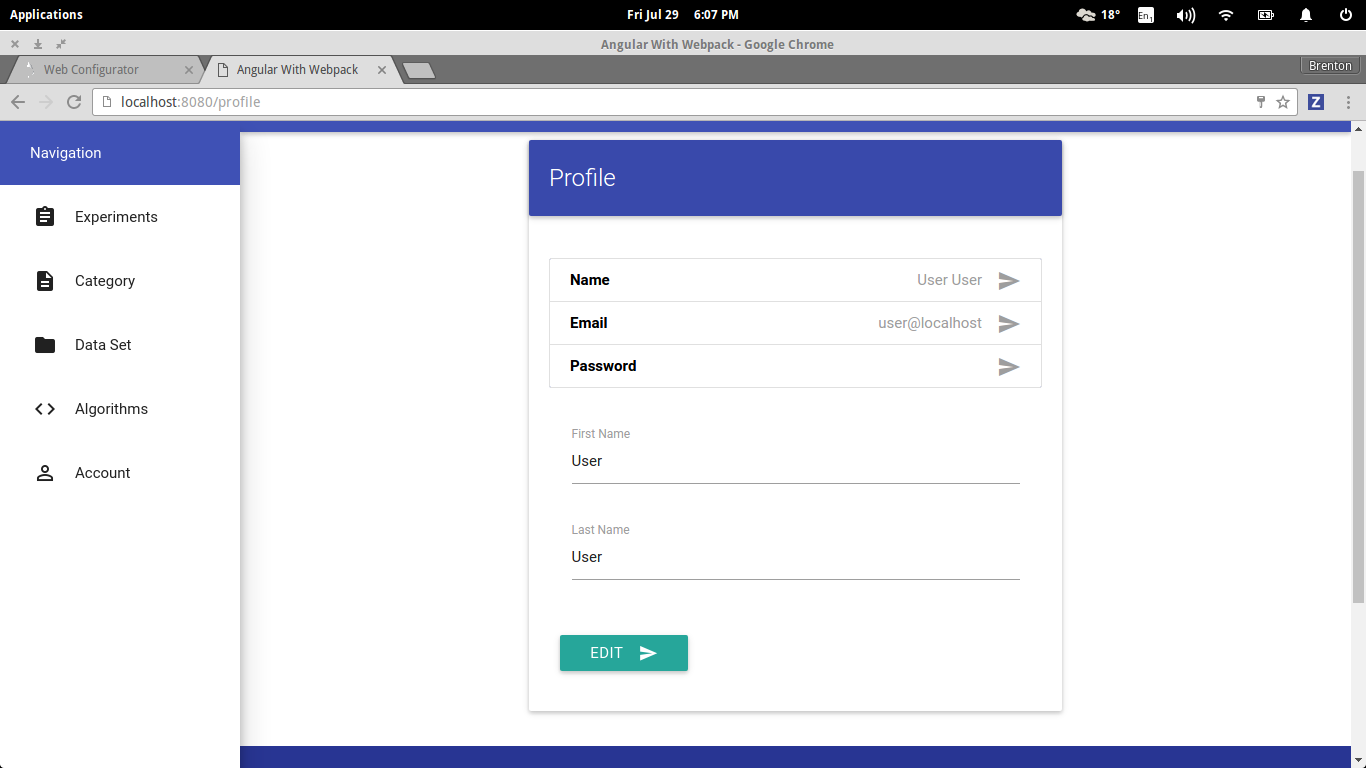
\includegraphics[scale=0.3]{../Images/User Manual/Profile Page1.png}
		\caption{Edit name}
		\label{fig:ProfilePage1}
	\end{center}  
\end{figure}
\begin{figure}[H]
	\begin{center}
		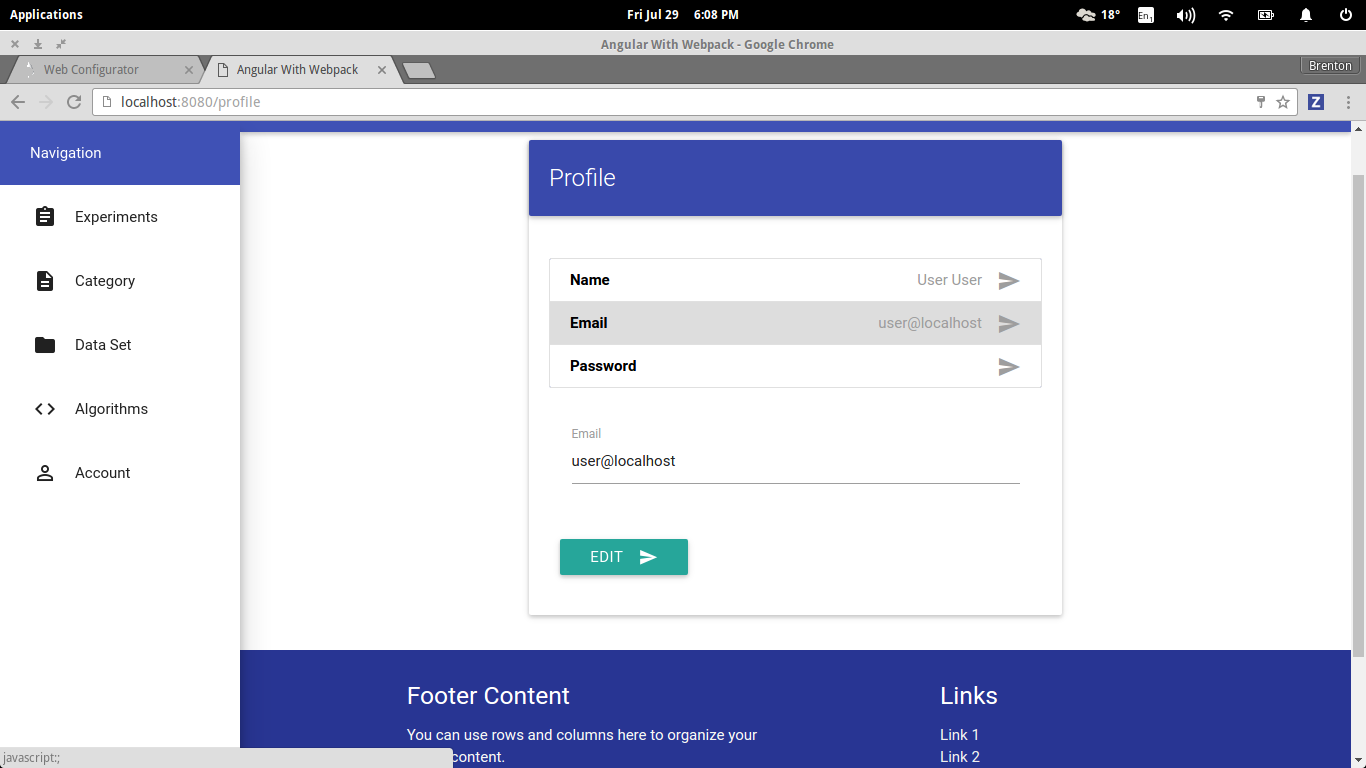
\includegraphics[scale=0.3]{../Images/User Manual/Profile Page2.png}
		\caption{Edit email}
		\label{fig:ProfilePage2}
	\end{center}  
\end{figure}
\begin{figure}[H]
	\begin{center}
		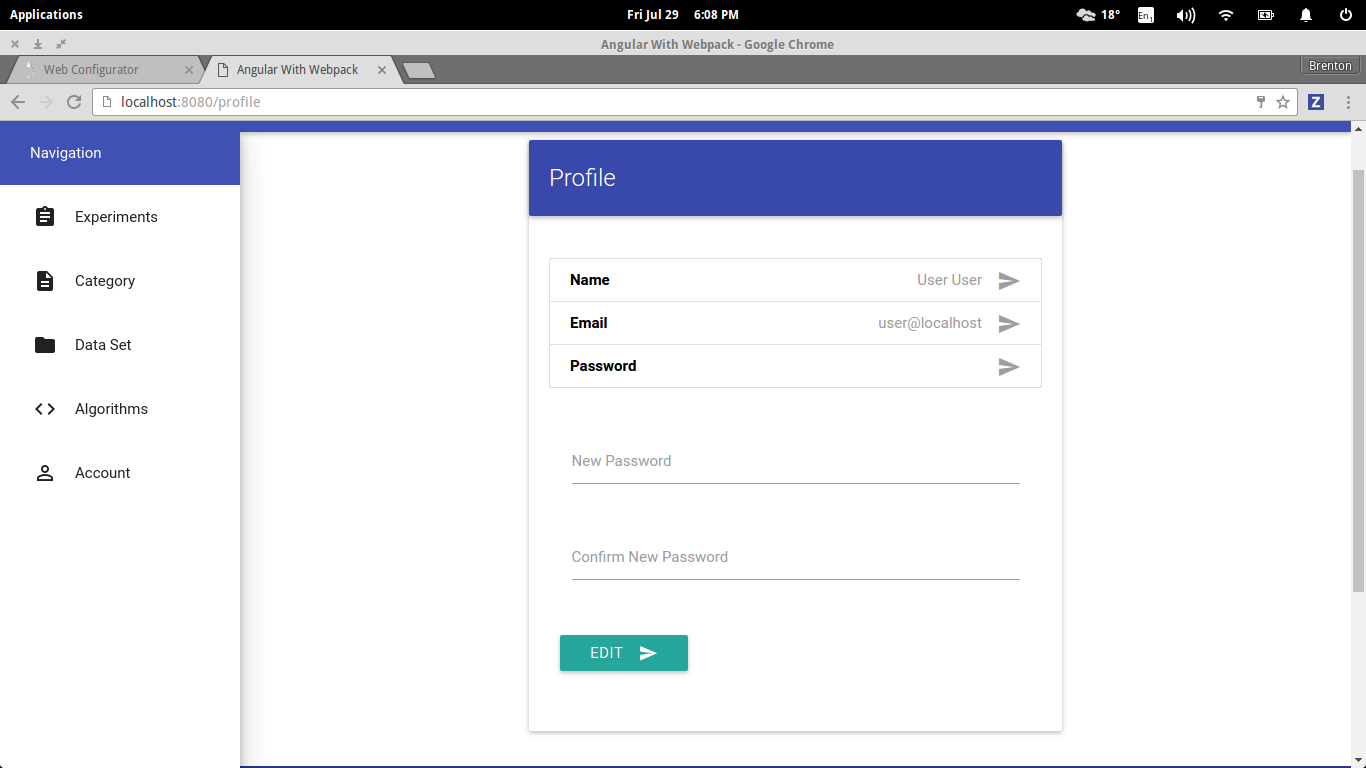
\includegraphics[scale=0.3]{../Images/User Manual/Profile Page3.png}
		\caption{Edit password}
		\label{fig:ProfilePage3}
	\end{center}  
\end{figure}

\section{Forgot password}
If one arrives at the landing page, and realizes they have lost or forgotten their password. They can select the
"Forgotten your password?" link at the bottom right which will take them to the page seen in Figure \ref{fig:forgotPage}.
\begin{figure}[H]
	\begin{center}
		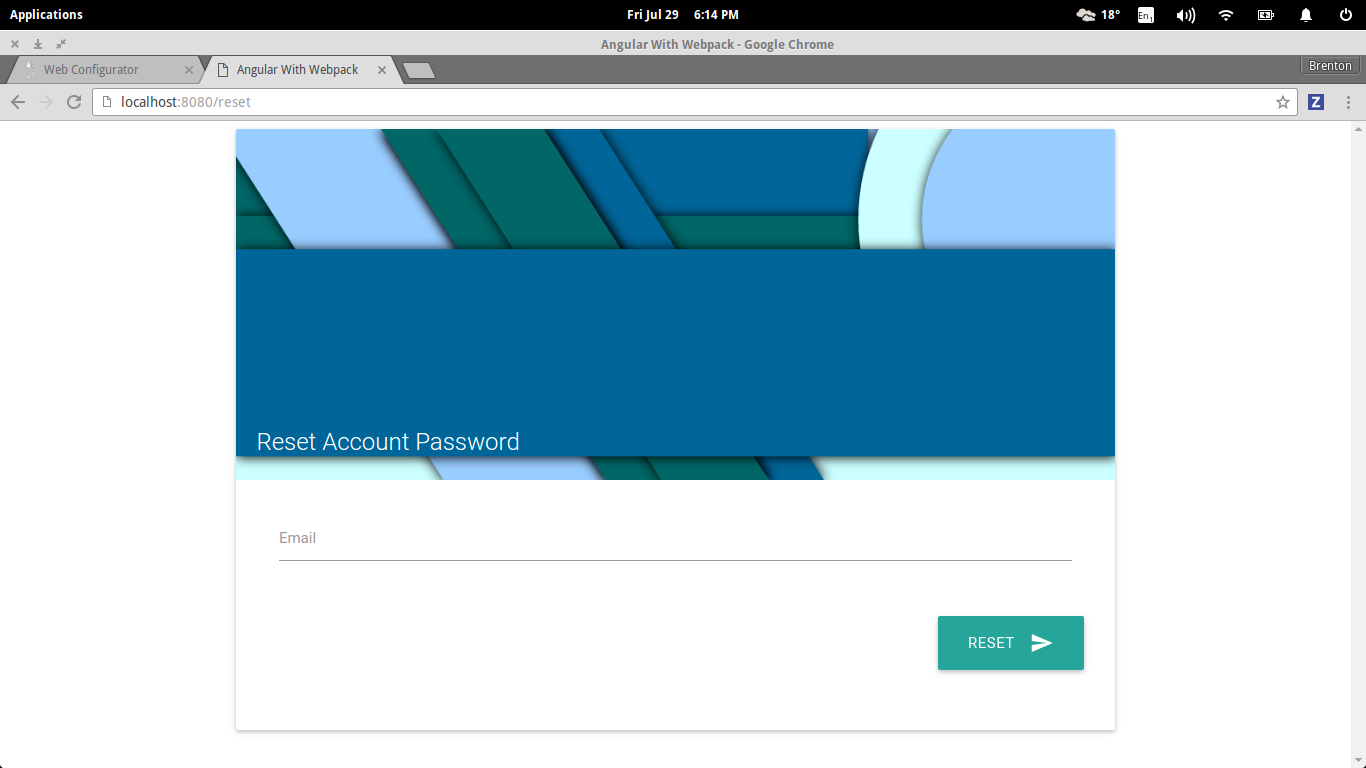
\includegraphics[scale=0.3]{../Images/User Manual/Forgot Page.png}
		\caption{Forgot password page}
		\label{fig:forgotPage}
	\end{center}  
\end{figure}
After entering their registered email address, the user will recieve an email with a link to a page to reset their password
as seen in Figure \ref{fig:resetPage}. After the user as filled in their details, the user should click "Reset".
\begin{figure}[H]
	\begin{center}
		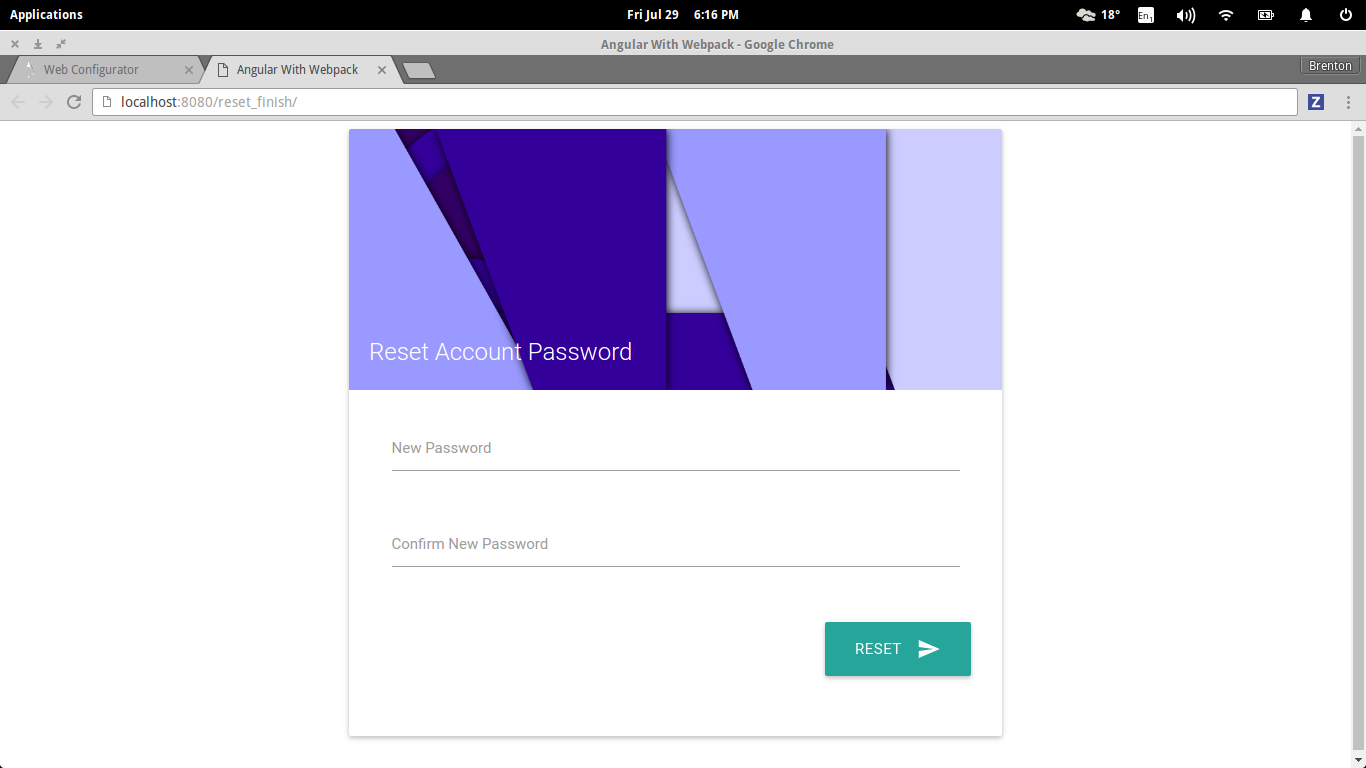
\includegraphics[scale=0.3]{../Images/User Manual/Reset Page.png}
		\caption{Reset password page}
		\label{fig:resetPage}
	\end{center}  
\end{figure}

\section{Experiment}
In order for a user to view their experiments the would navigate to the View Experiments
page as seen in Figure \ref{fig:viewExperiments} and a list of all current experiments 
being run or that have been run for the user will be displayed. The user can click on
an individual experiment to see more detail surrounding the experiment as seen in 
Figure \ref{fig:viewExperiment}. If the test has finished executing a chart will display
providing the user with a quick graphical representation of their results.
\begin{figure}[H]
	\begin{center}
		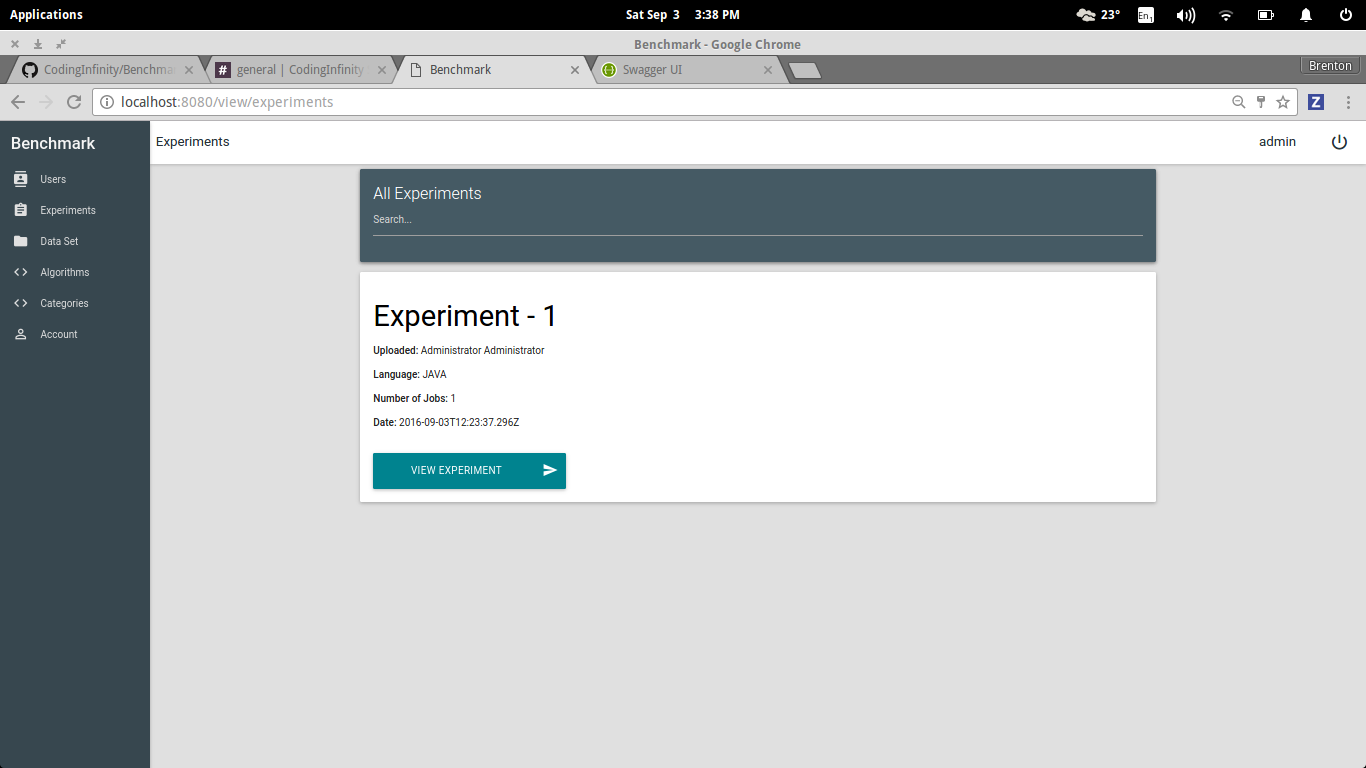
\includegraphics[scale=0.3]{../Images/User Manual/View Experiments.png}
		\caption{View Experiments page}
		\label{fig:viewExperiments}
	\end{center}  
\end{figure}

\begin{figure}[H]
	\begin{center}
		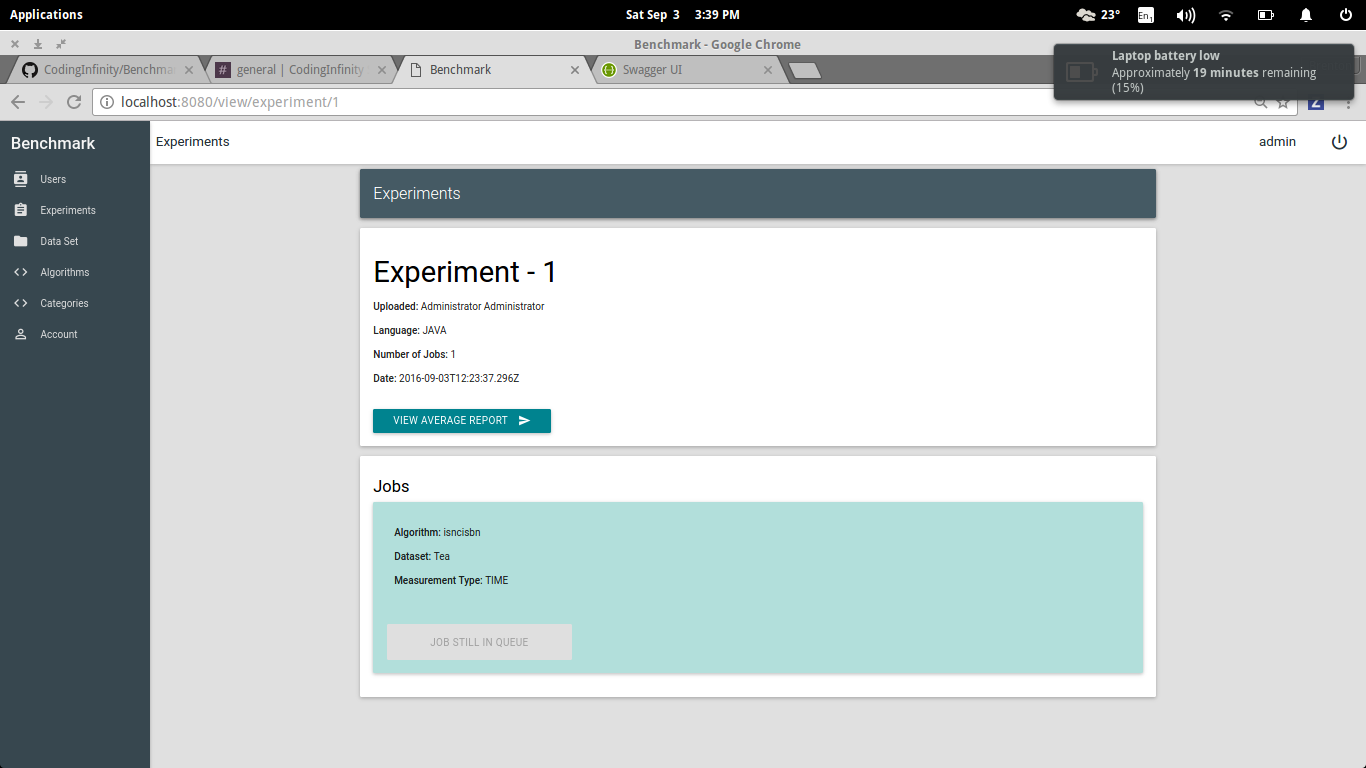
\includegraphics[scale=0.3]{../Images/User Manual/View Experiment.png}
		\caption{View experiment page}
		\label{fig:viewExperiment}
	\end{center}  
\end{figure}

\section{Category}
In order for a user to view this section they need to be logged in as an administrator.
By clicking the category drop down item in the navigation menu, the user has access to
view all algorithm categories as seen in Figure \ref{fig:viewAlCat}, create new algorithm
categories as seen in Figure \ref{fig:createAlCat}, view all dataset categories as seen in
Figure \ref{fig:viewDataCat} and create new dataset categories as seen in Figure \ref{fig:createDataCat}.
On the respective viewing pages, a user can delete and edit certain categories.

\begin{figure}[H]
	\begin{center}
		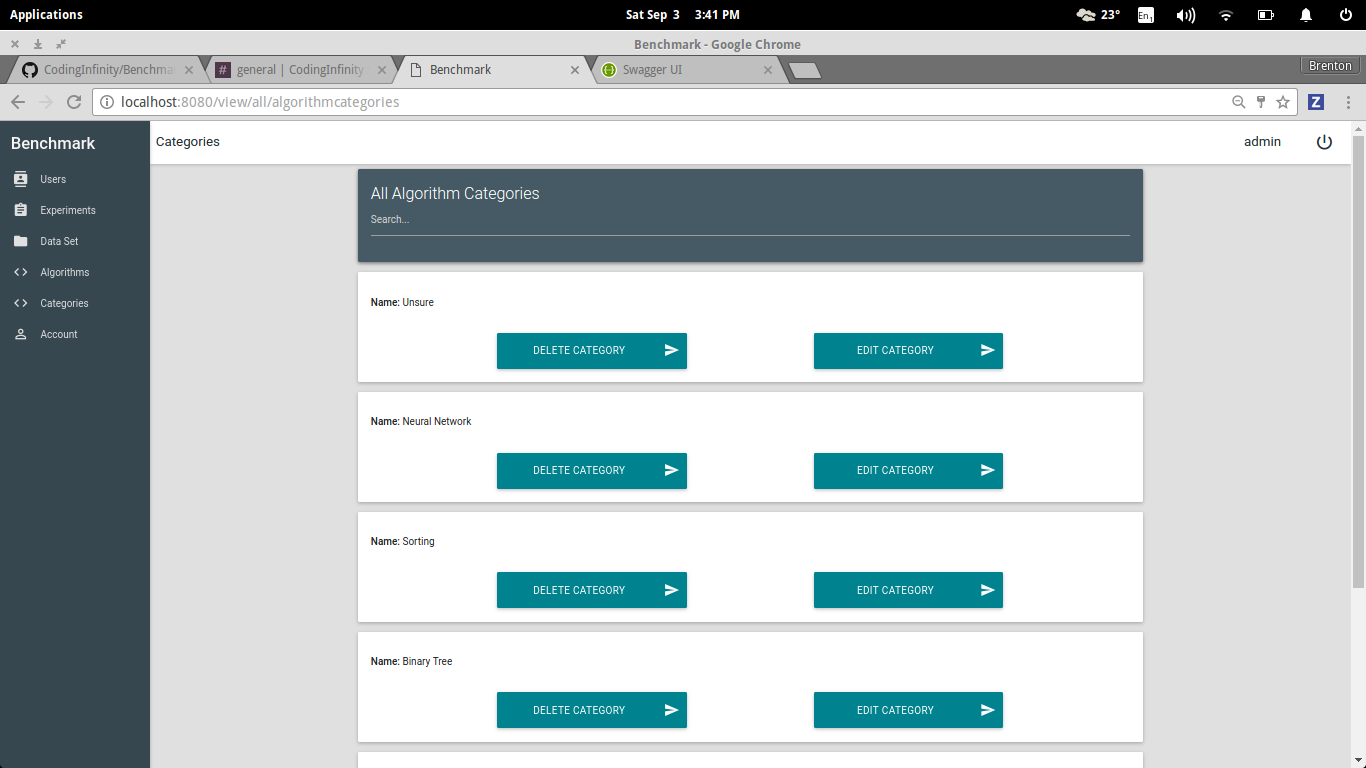
\includegraphics[scale=0.3]{../Images/User Manual/View Algorithm Categories.png}
		\caption{View all algorithm categories page}
		\label{fig:viewAlCat}
	\end{center}  
\end{figure}
\begin{figure}[H]
	\begin{center}
		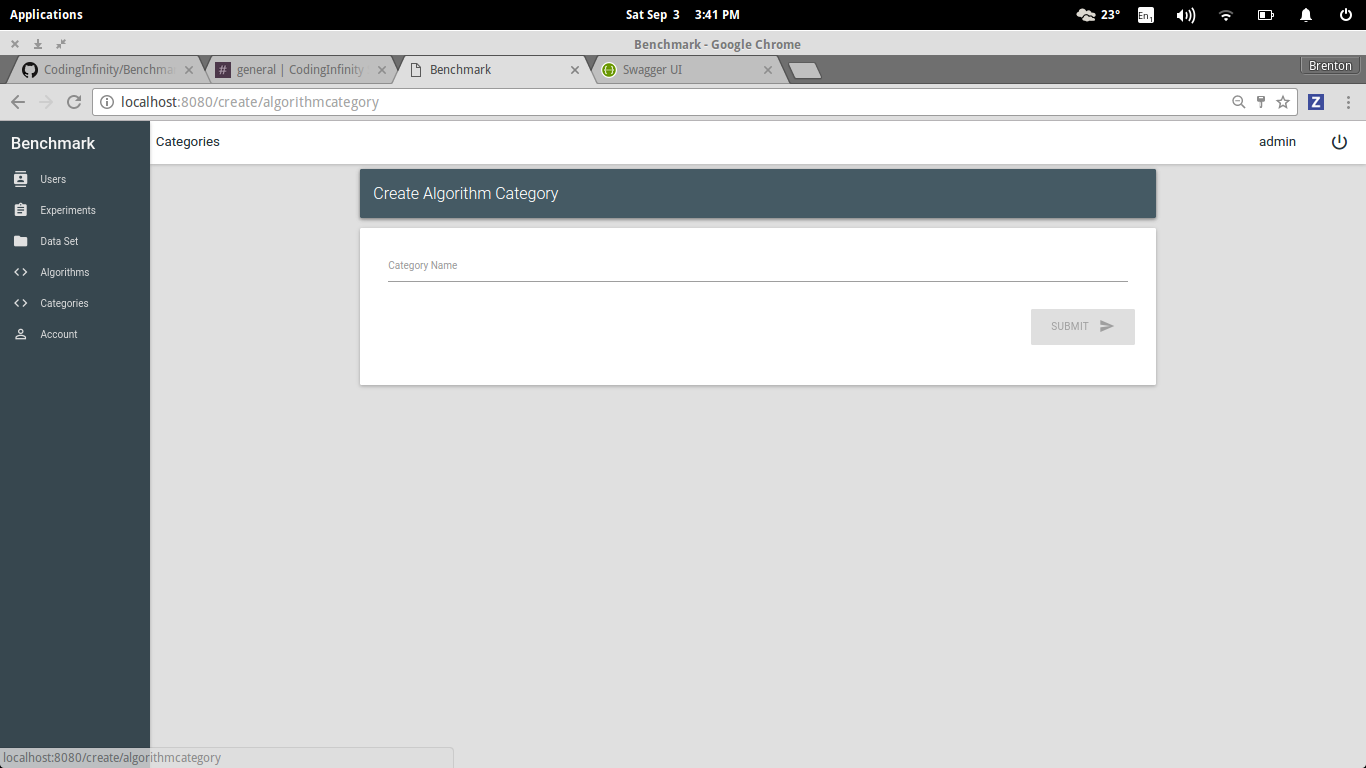
\includegraphics[scale=0.3]{../Images/User Manual/Create Algorithm Category.png}
		\caption{Create algorithm category page}
		\label{fig:createAlCat}
	\end{center}  
\end{figure}
\begin{figure}[H]
	\begin{center}
		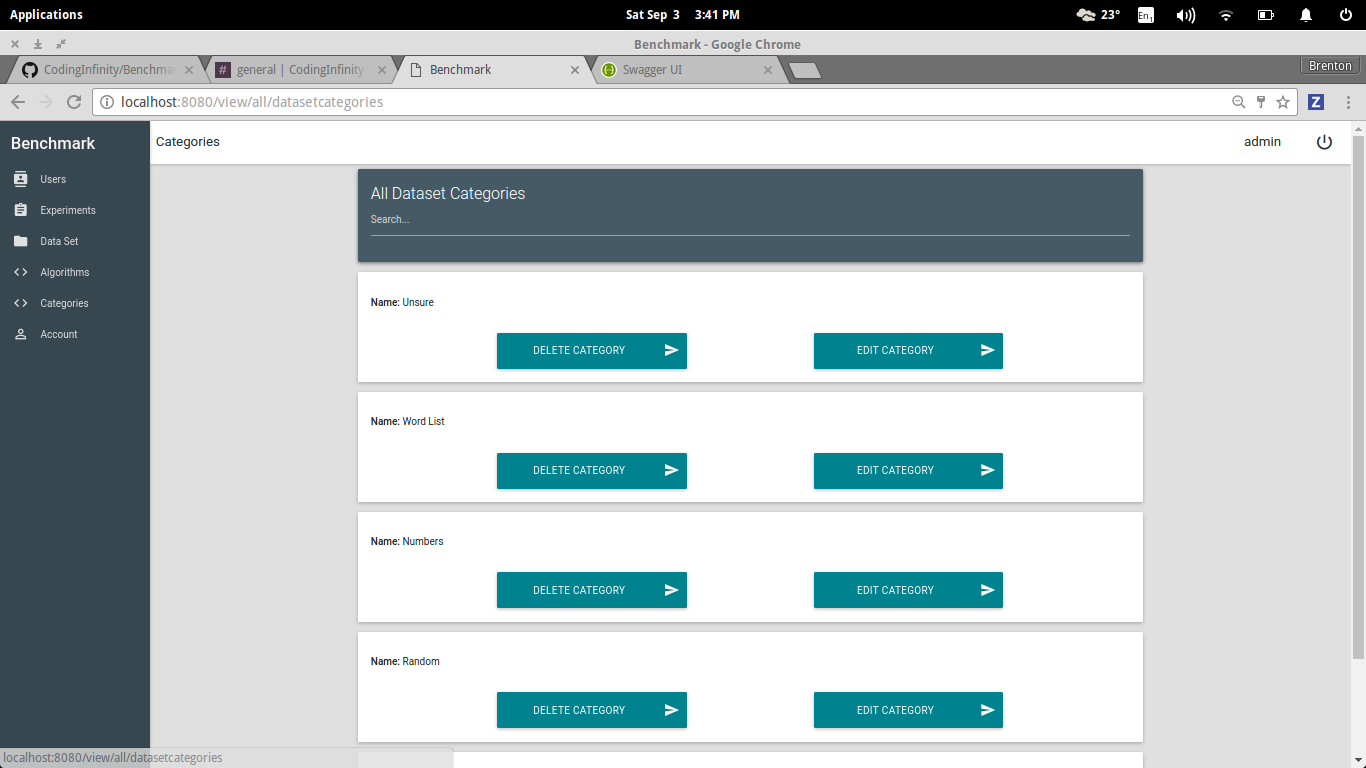
\includegraphics[scale=0.3]{../Images/User Manual/View Dataset Categories.png}
		\caption{View all dataset categories page}
		\label{fig:viewDataCat}
	\end{center}  
\end{figure}
\begin{figure}[H]
	\begin{center}
		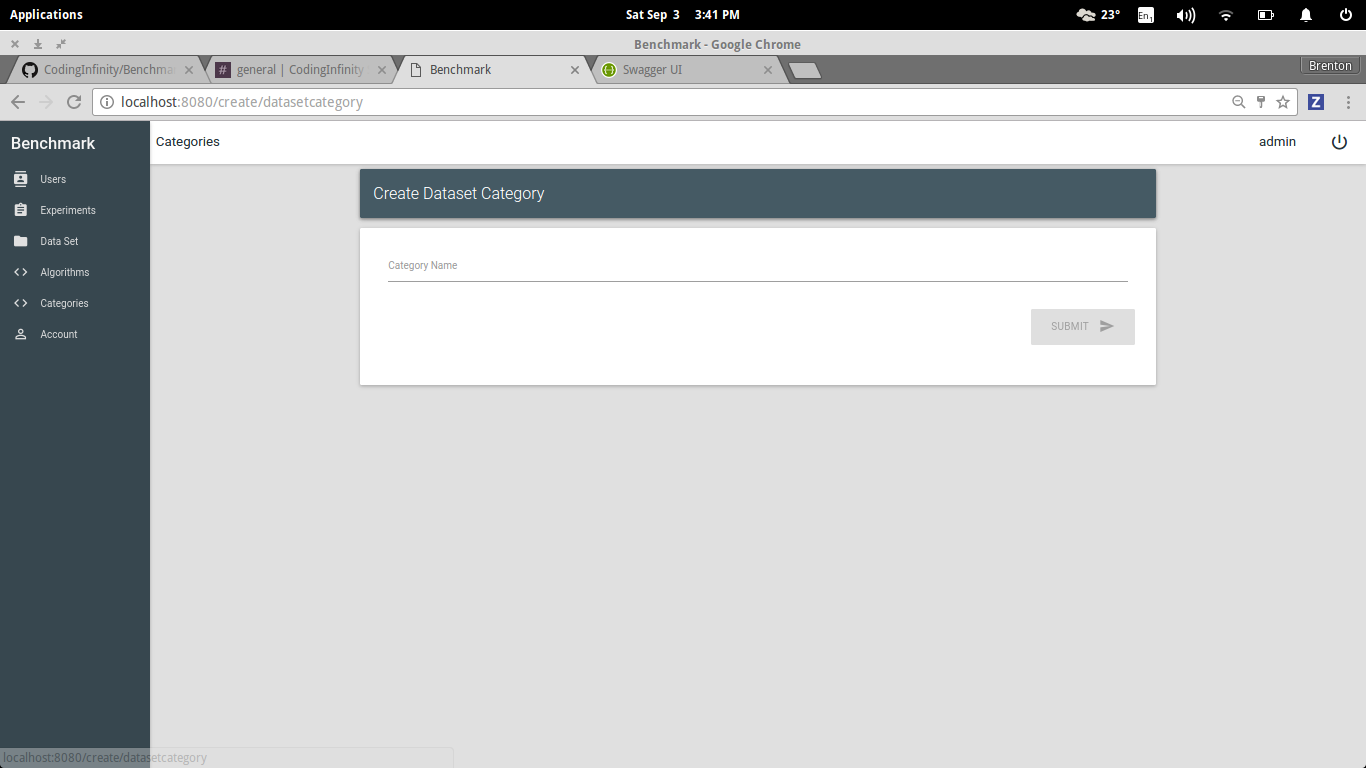
\includegraphics[scale=0.3]{../Images/User Manual/Create Dataset Category.png}
		\caption{Create dataset category page}
		\label{fig:createDataCat}
	\end{center}  
\end{figure}

\section{Dataset}
This section can be accessed by expanding the data set item in the navigation bar, from
here a user has the ability to navigate to pages that will allow them to view all data
sets as seen in Figure \ref{fig:viewAllData} or simply view the data sets they have
created as seen in Figure \ref{fig:viewUserData} from either of these pages they can choose
to view the data set in more detail as seen in \ref{fig:viewData} or they can upload a new
data set as seen in Figure \ref {fig:createData}.

\begin{figure}[H]
	\begin{center}
		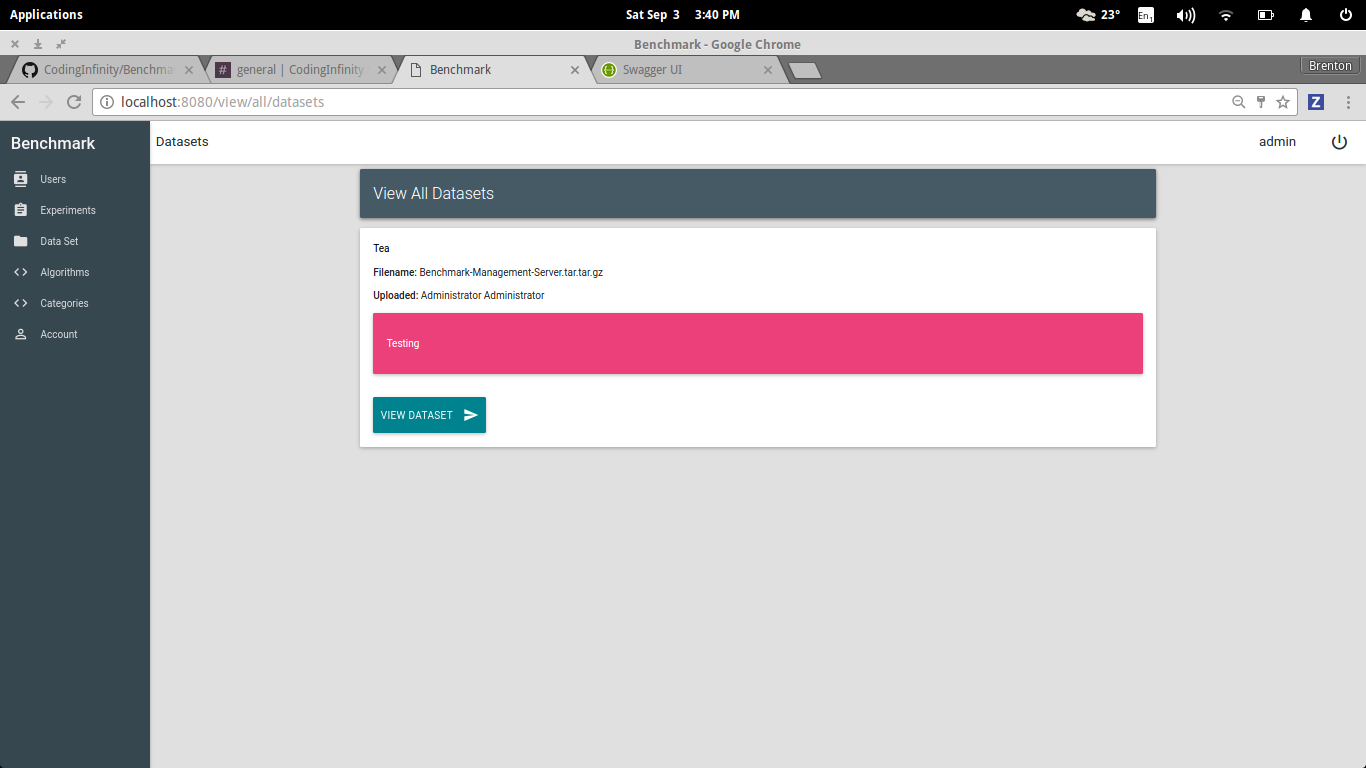
\includegraphics[scale=0.3]{../Images/User Manual/View All Datasets.png}
		\caption{View all datasets page}
		\label{fig:viewAllData}
	\end{center}  
\end{figure}
\begin{figure}[H]
	\begin{center}
		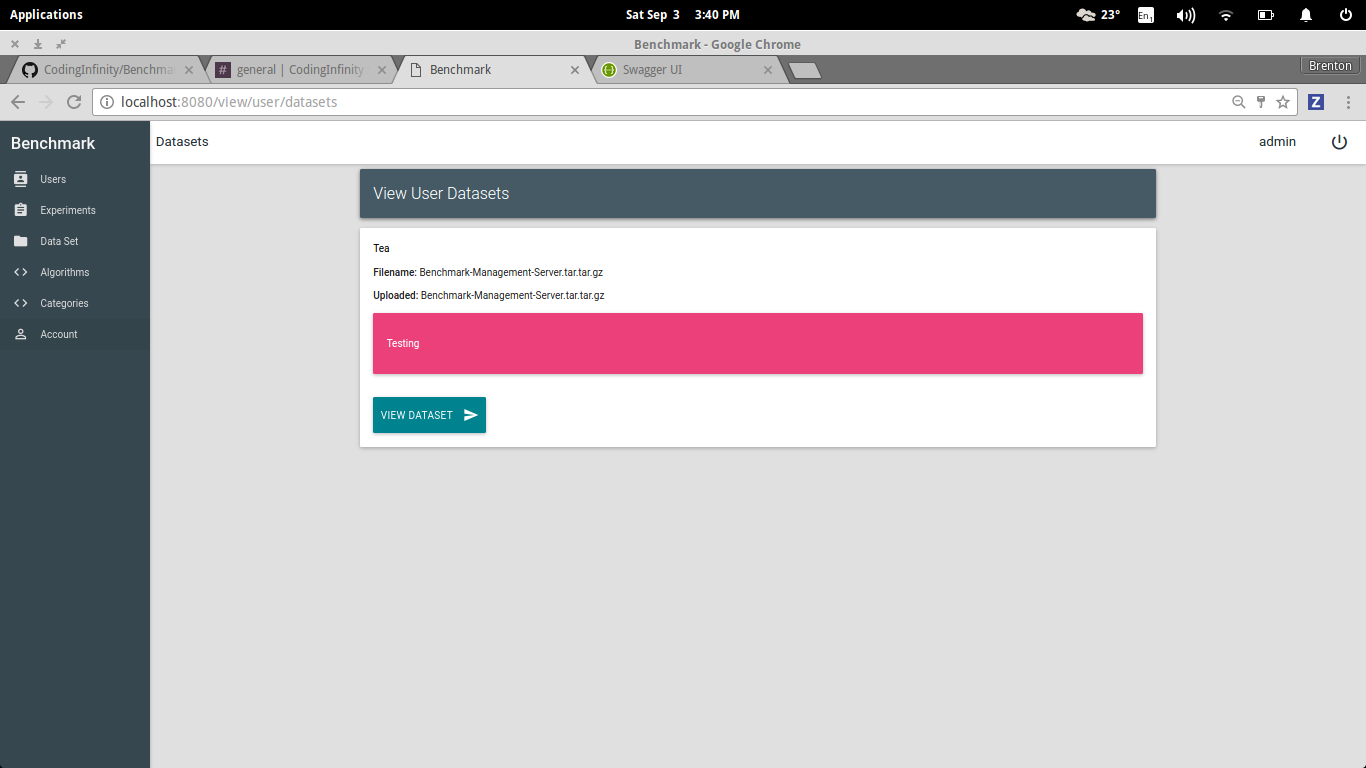
\includegraphics[scale=0.3]{../Images/User Manual/View User Datasets.png}
		\caption{View user datasets page}
		\label{fig:viewUserData}
	\end{center}  
\end{figure}
\begin{figure}[H]
	\begin{center}
		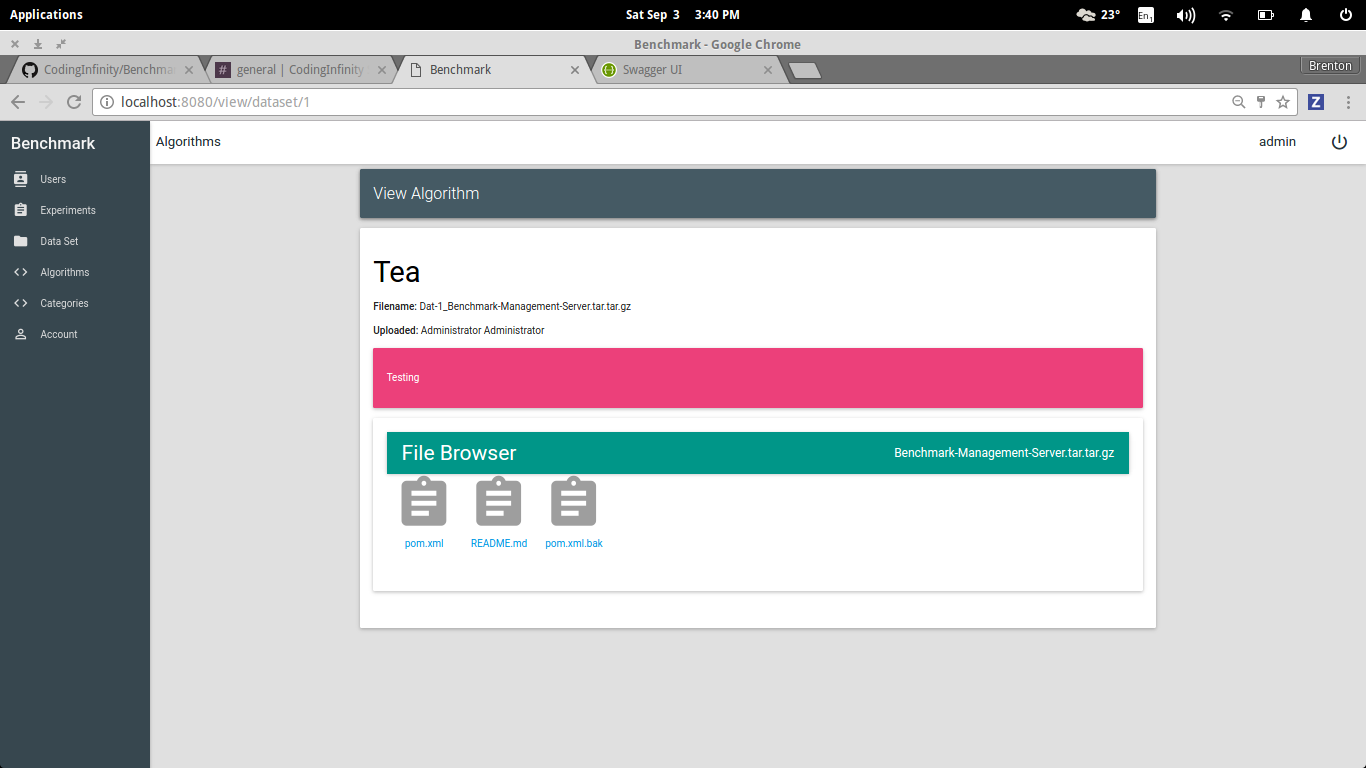
\includegraphics[scale=0.3]{../Images/User Manual/View Dataset.png}
		\caption{View dataset page}
		\label{fig:viewData}
	\end{center}  
\end{figure}
\begin{figure}[H]
	\begin{center}
		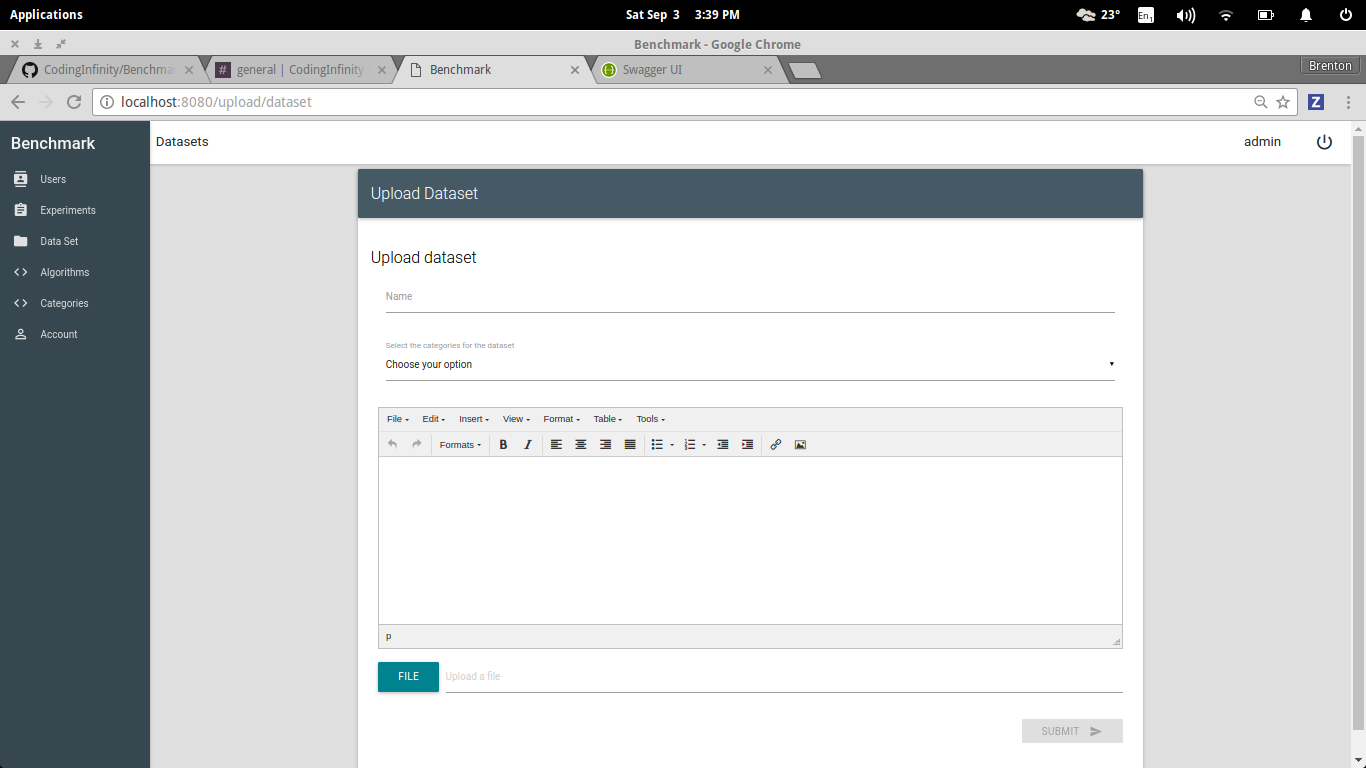
\includegraphics[scale=0.3]{../Images/User Manual/Upload Dataset.png}
		\caption{Create dataset page}
		\label{fig:createData}
	\end{center}  
\end{figure}

\section{Algorithms}
This section can be accessed by expanding the algorithm item in the navigation bar, from
here a user has the ability to navigate to pages that will allow them to view all algorithms
as seen in Figure \ref{fig:viewAllAlg} or simply view the algorithms they have
created as seen in Figure \ref{fig:viewUserAlg} from either of these pages they can choose
to view the algorithm in more detail as seen in \ref{fig:viewAlg} or they can upload a new
algorithm as seen in Figure \ref {fig:createAlg}.

\begin{figure}[H]
	\begin{center}
		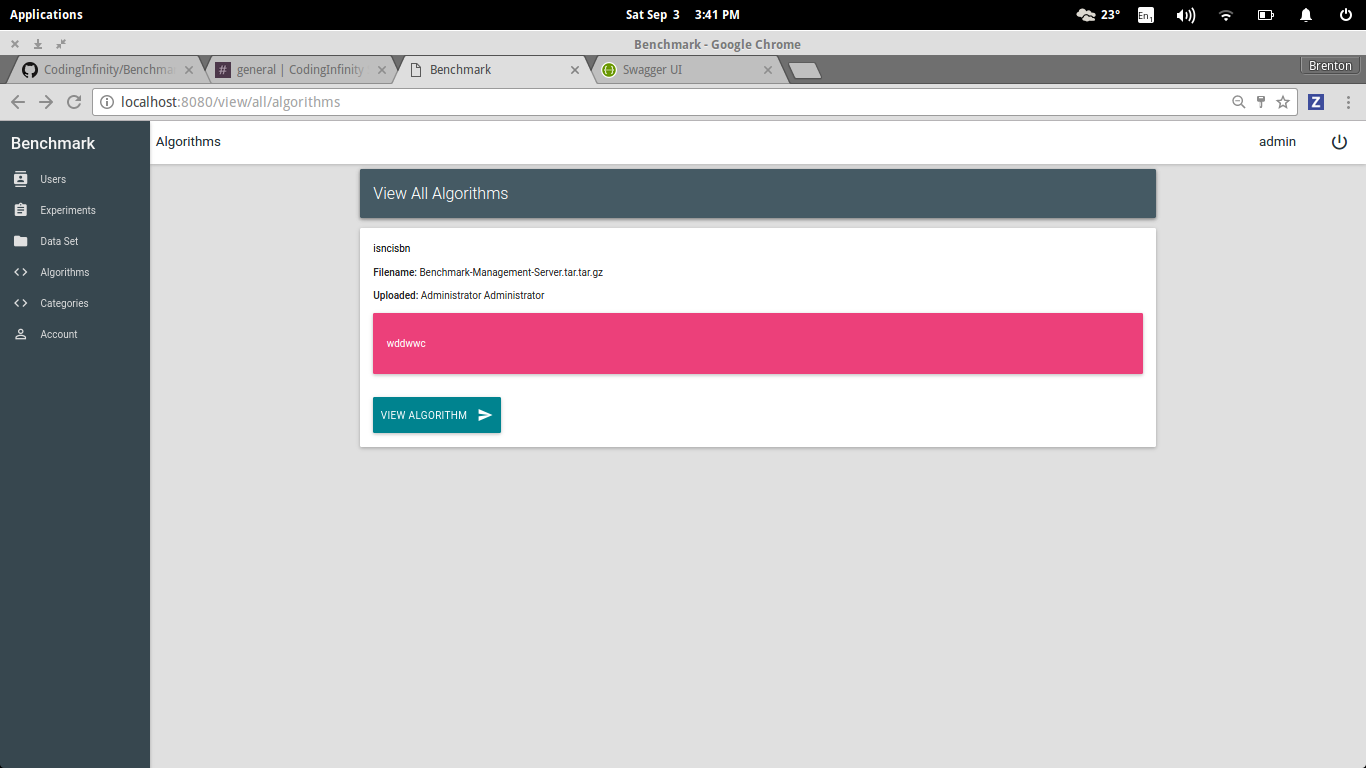
\includegraphics[scale=0.3]{../Images/User Manual/View Algorithms.png}
		\caption{View all algorithms page}
		\label{fig:viewAllAlg}
	\end{center}  
\end{figure}
\begin{figure}[H]
	\begin{center}
		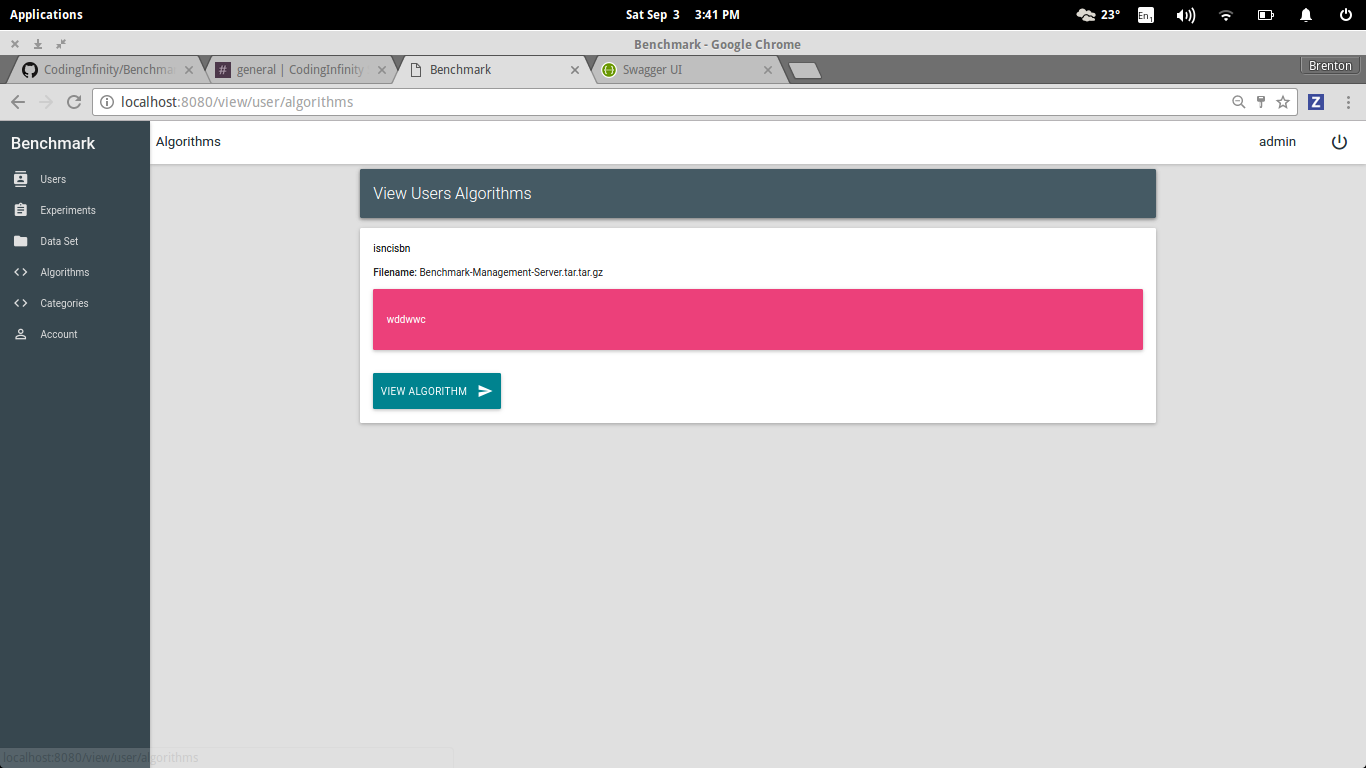
\includegraphics[scale=0.3]{../Images/User Manual/View User Algorithms.png}
		\caption{View user algorithm page}
		\label{fig:viewUserAlg}
	\end{center}  
\end{figure}
\begin{figure}[H]
	\begin{center}
		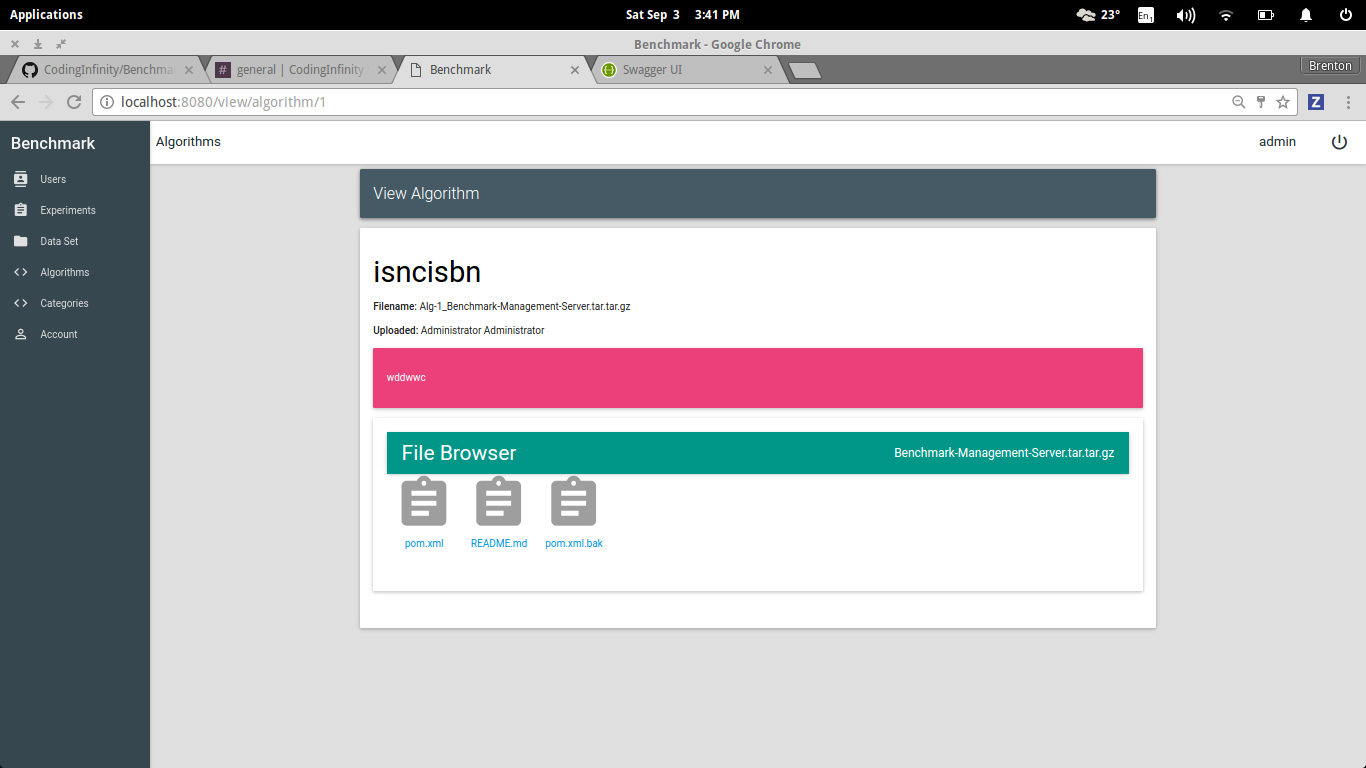
\includegraphics[scale=0.3]{../Images/User Manual/View Algorithm.png}
		\caption{View algorithm page}
		\label{fig:viewAlg}
	\end{center}  
\end{figure}
\begin{figure}[H]
	\begin{center}
		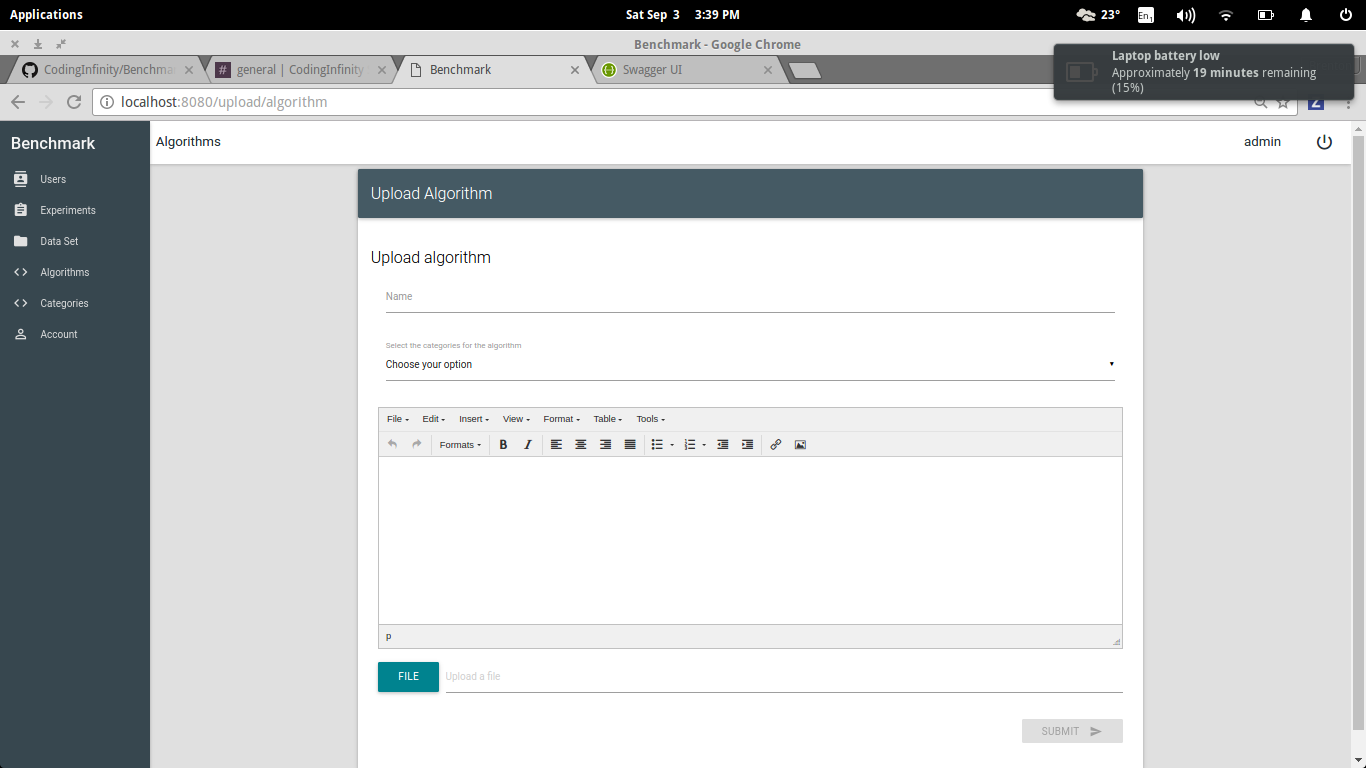
\includegraphics[scale=0.3]{../Images/User Manual/Upload Algorithm.png}
		\caption{Create algorithm page}
		\label{fig:createAlg}
	\end{center}  
\end{figure}
\end{document}
